\documentclass[conference]{IEEEtran}
\usepackage{graphicx} % Required for inserting images
\usepackage{float}
\usepackage{subcaption}
\usepackage{hyperref}

\def\BibTeX{{\rm B\kern-.05em{\sc i\kern-.025em b}\kern-.08em
    T\kern-.1667em\lower.7ex\hbox{E}\kern-.125emX}}
\begin{document}

\title{Data Mining Project: Analyzing Video Game Sales\\
{\footnotesize \textsuperscript{*} CS 4412: Data Mining}

}

\author{\IEEEauthorblockN{Joshua Vach}
\IEEEauthorblockA{\textit{Student at Kennesaw State University} \\
Marietta GA \\
jvach3@students.kennesaw.edu}

}
\maketitle

\section{Introduction} This project is focused on analyzing sales of various video games and the trends that appear within this data. It will focus on sales trends across various different markets and analyze how they effect game sale performance in various markets and the global stage.
\subsection{Data Set}
\subsubsection*{Link to Data Set} \url{https://www.kaggle.com/datasets/gregorut/videogamesales/data}

The data set has 16600 rows, which means
that 16600 games are in the data set, and 11 columns,
each game has a unique rank assigned to it that is ranked
from highest selling to lowest selling. The data set is
stored in CSV format and is 1.36 megabytes The attributes that will be used aside from the name of the game consist of Rank, Platform, Year, Genre,
Publisher,NASales, EUSales, JPSales, OtherSales and GlobalSales 

There are several issues with this dataset the most apparent is that it is several years out of date so it only contains one game past 2017 which is from 2020. There are also many games that do not contain data for various data points. The data set also does not count sales past its last update and since many games on this list are still on the market the sales could be slightly off. There is also a lack of multiple important video game markets like Korea and China which could skew results.
\subsection{Exploratory Data Analysis}
We did several exploratory data in order to find out a baseline for trends happening in the game industry over time.
\subsubsection{Video Game Releases per Year}
The first data analysis is the amount of games released per year to show the growth of the games industry over time. It shows a clear trend of increasing sales from the mid 90s to around 2010 then a fall off in sales around 2010.


\begin{figure}[H]
    \centering
    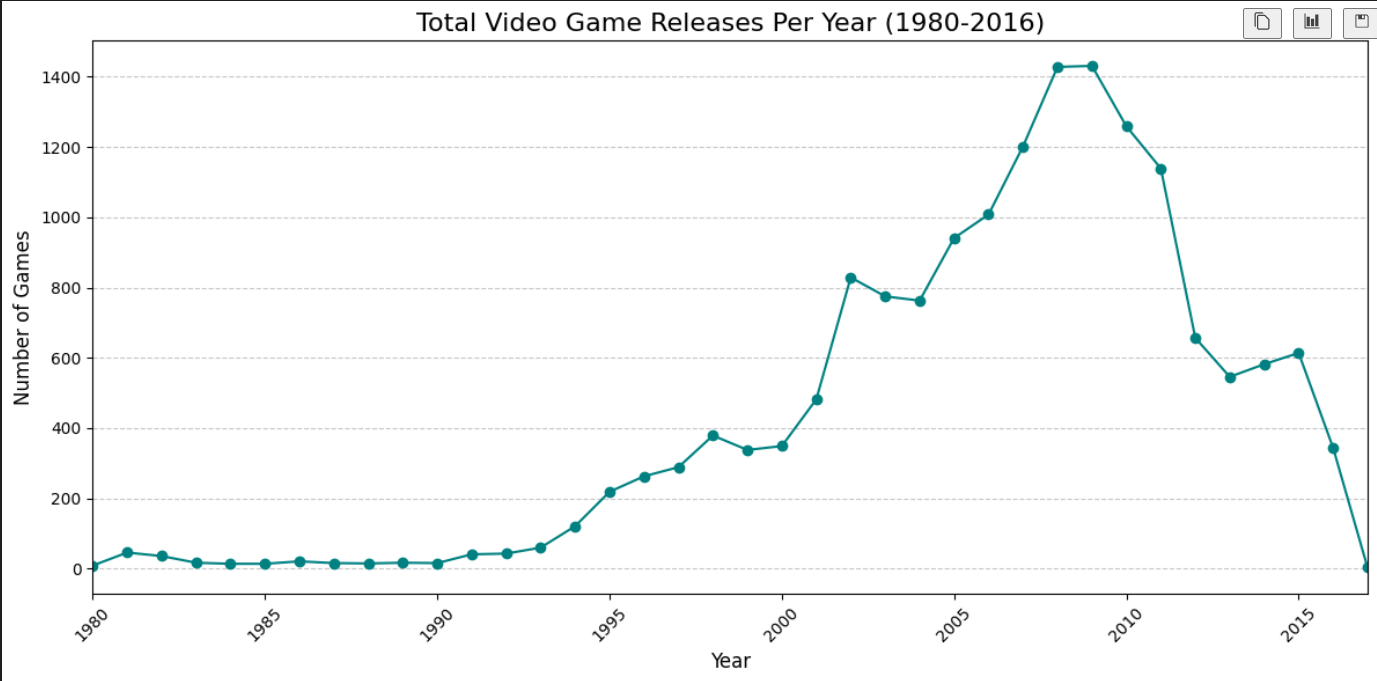
\includegraphics[width=0.8\linewidth]{vgreleases.png}
    \label{fig:placeholder}
\end{figure}

\subsubsection{Top Publishers, Genre, and Platform by releases}
We analyzed several different data points in the dataset in order to find the top genre publishers and platform in  order to find broad trends based on this data. We found that the DS and PS2 were dominant in the platform department and EA is dominant in the publishing department while Action and Sports are the two largest genres by a wide margin.
\begin{figure}[H]
    \centering
    \begin{subfigure}[b]{0.2\textwidth}
        \centering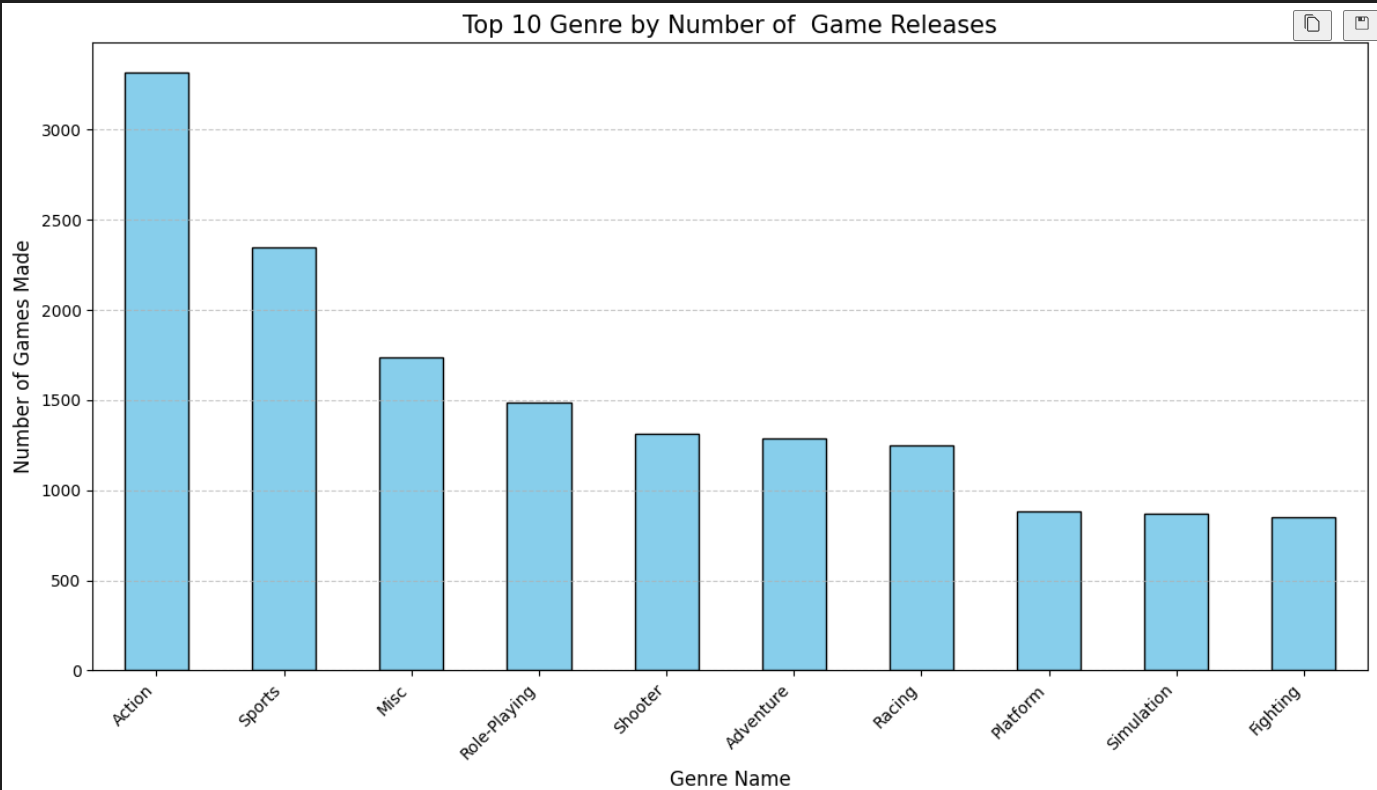
\includegraphics[width=\textwidth]{vggenre.png}
    \end{subfigure}
    \hfill
    \begin{subfigure}[b]{0.2\textwidth}
        \centering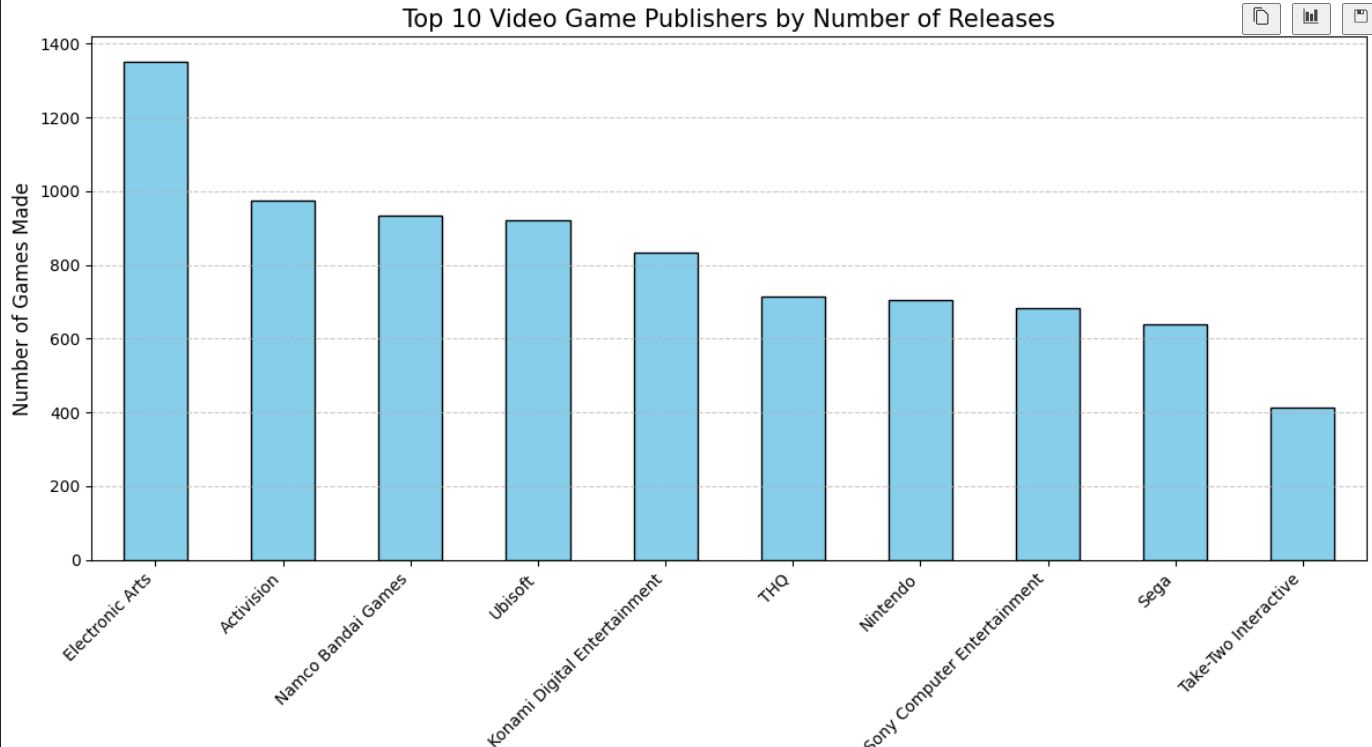
\includegraphics[width=\textwidth]{vgpublish.png}
    \end{subfigure}
    \hfill
    \begin{subfigure}[b]{0.2\textwidth}
        \centering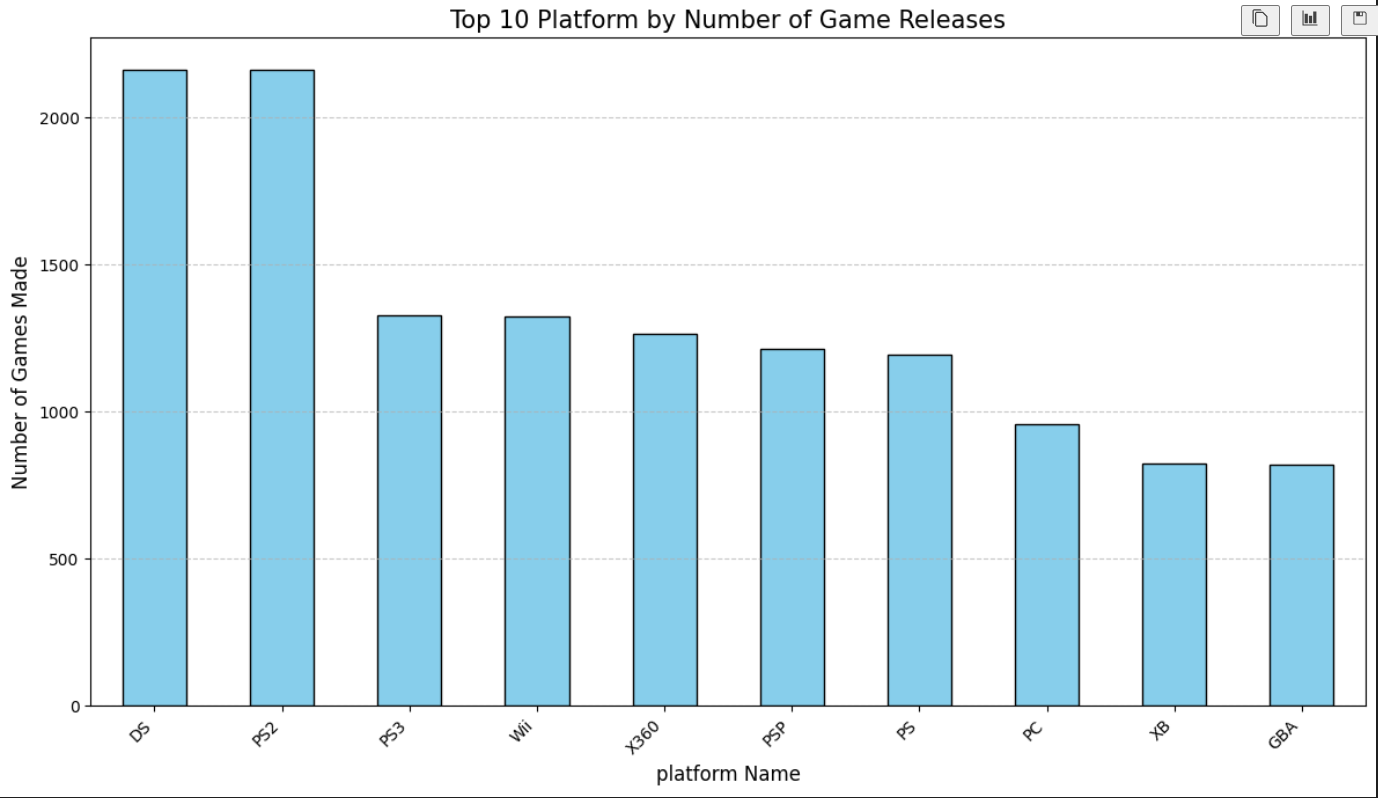
\includegraphics[width=\textwidth]{vgsalesplat.png}
    \end{subfigure}
\end{figure}


\subsubsection{Sales Trend by Region}
We also analyzed the total sales both globally and in the major markets in order to get an overview of how sales have changed in the various markets over time. While other markets have increased in sales massively in the 90s and 2000s Japan remained stable and even started declining earlier than the other markets.

\begin{figure}[H]
    \centering
    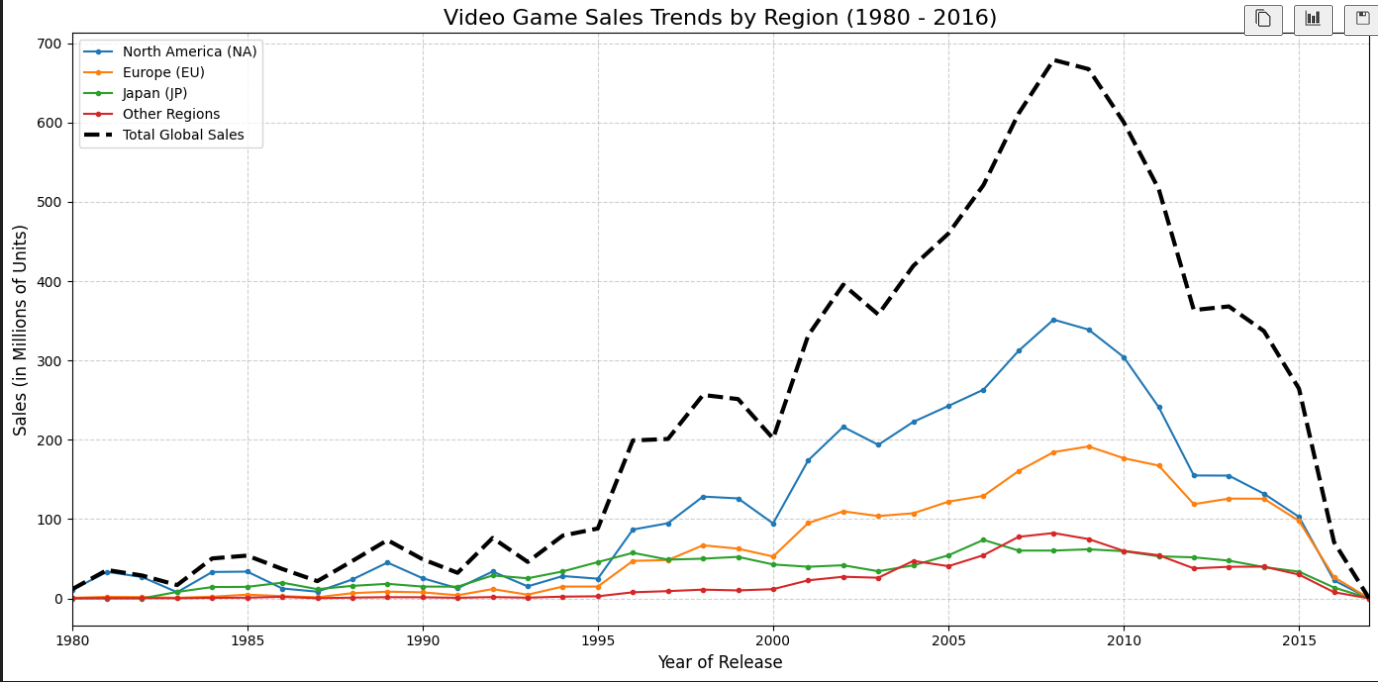
\includegraphics[width=0.8\linewidth]{vgsalesregion.png}
    \label{fig:placeholder}
\end{figure}

\subsubsection{Sales Comparison by Region for Publishers and Platforms}
In order to properly analyze how each platform and publisher does in every market to see if the home market of the publisher/platform has any effect on its performance in other markets. Non-Japanese Companies tend to struggle in the Japanese market while Japanese companies tend to also do well outside of Japan especially inside North America.
\begin{figure}[H]
    \centering
    \begin{subfigure}[b]{0.2\textwidth}
        \centering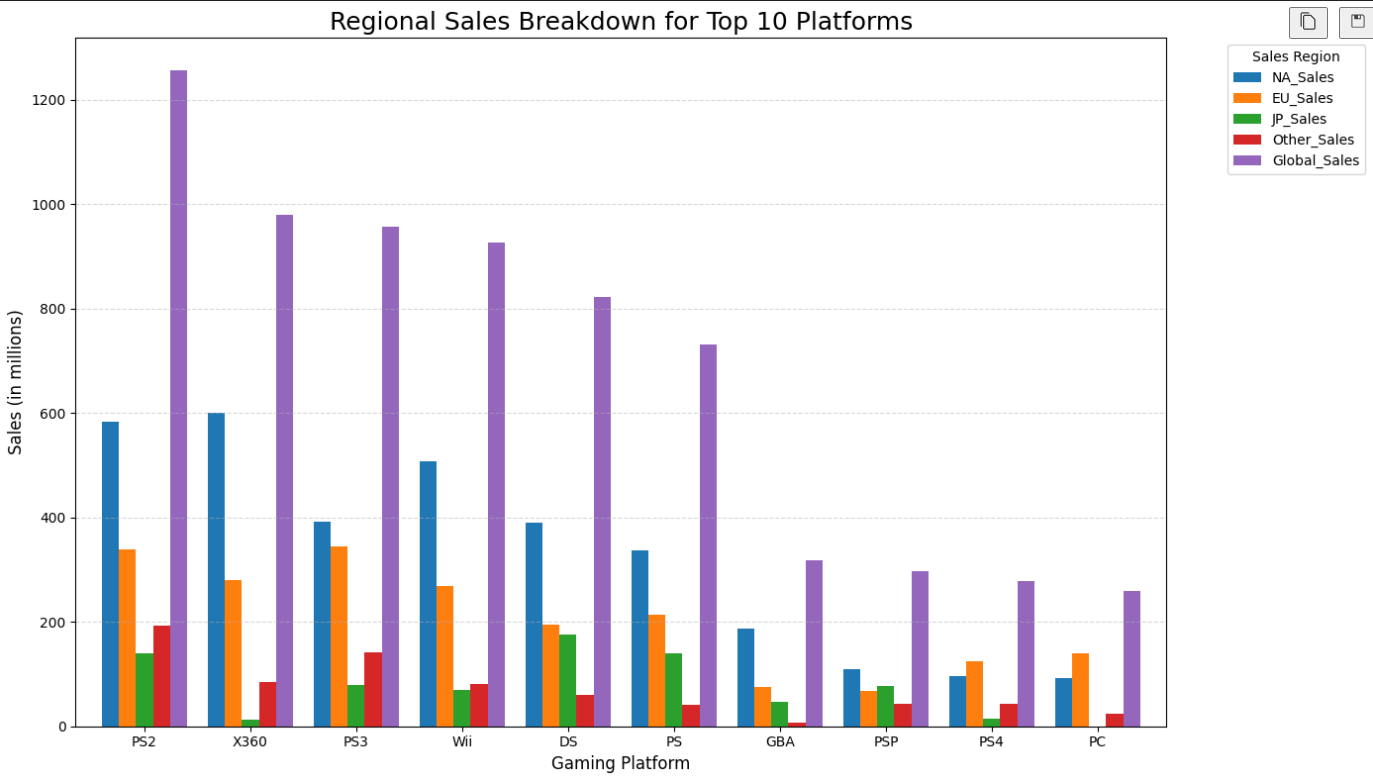
\includegraphics[width=\textwidth]{vgsalesplatform.png}
    \end{subfigure}
    \hfill
    \begin{subfigure}[b]{0.2\textwidth}
        \centering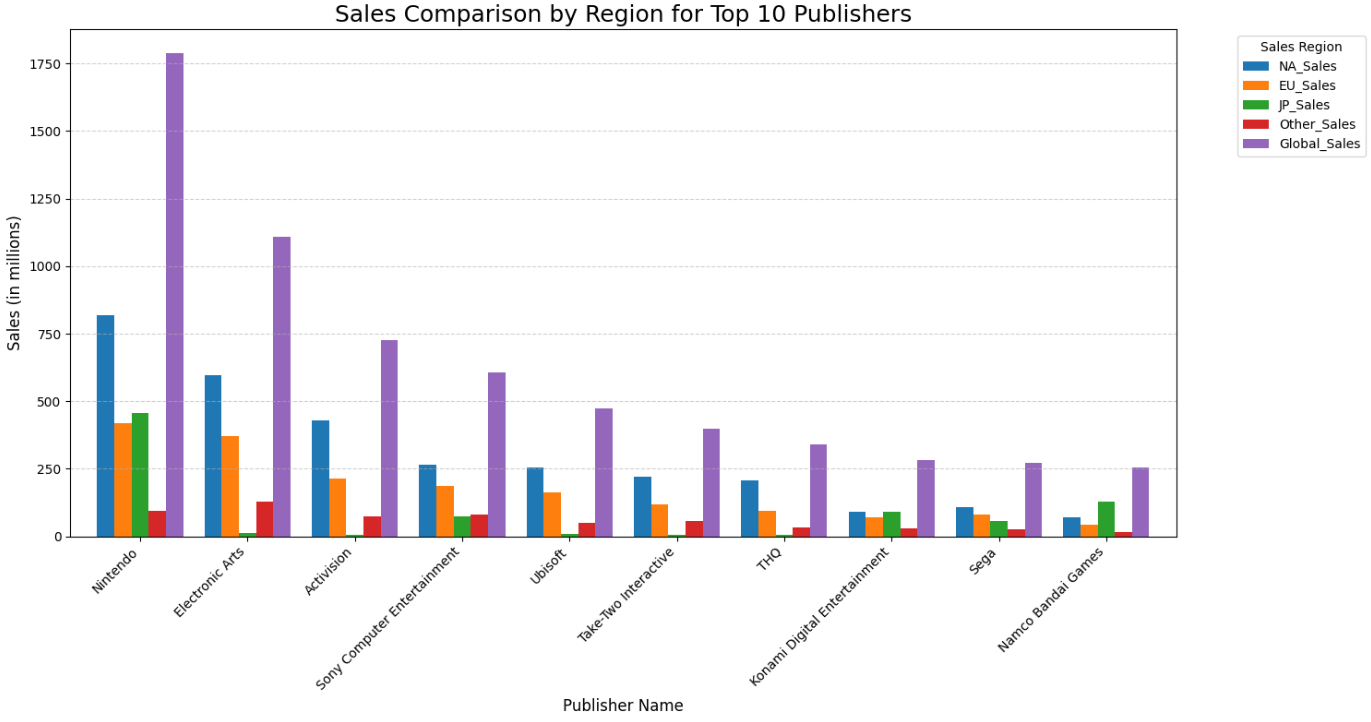
\includegraphics[width=\textwidth]{vgsalespublisher.png}
    \end{subfigure}
\end{figure}

\subsubsection{Sales Comparison of top 10 Platforms and Publisher over time}
Tracking and Analyzing how sales of various publishers and platforms perform over time can show changes in consumer sentiment as well as show which publishers do better when each platform is most popular. Nintendo dominates with sales especially during the era where the Wii was the most popular console which is likely due to them publishing most games that are on their own consoles while sony allows other publishers to publish on their consoles. This allows other publishers to sell well even when Sony consoles are dominating the market compared to when Nintendo consoles are.

\begin{figure}[H]
    \centering
    \begin{subfigure}[b]{0.2\textwidth}
        \centering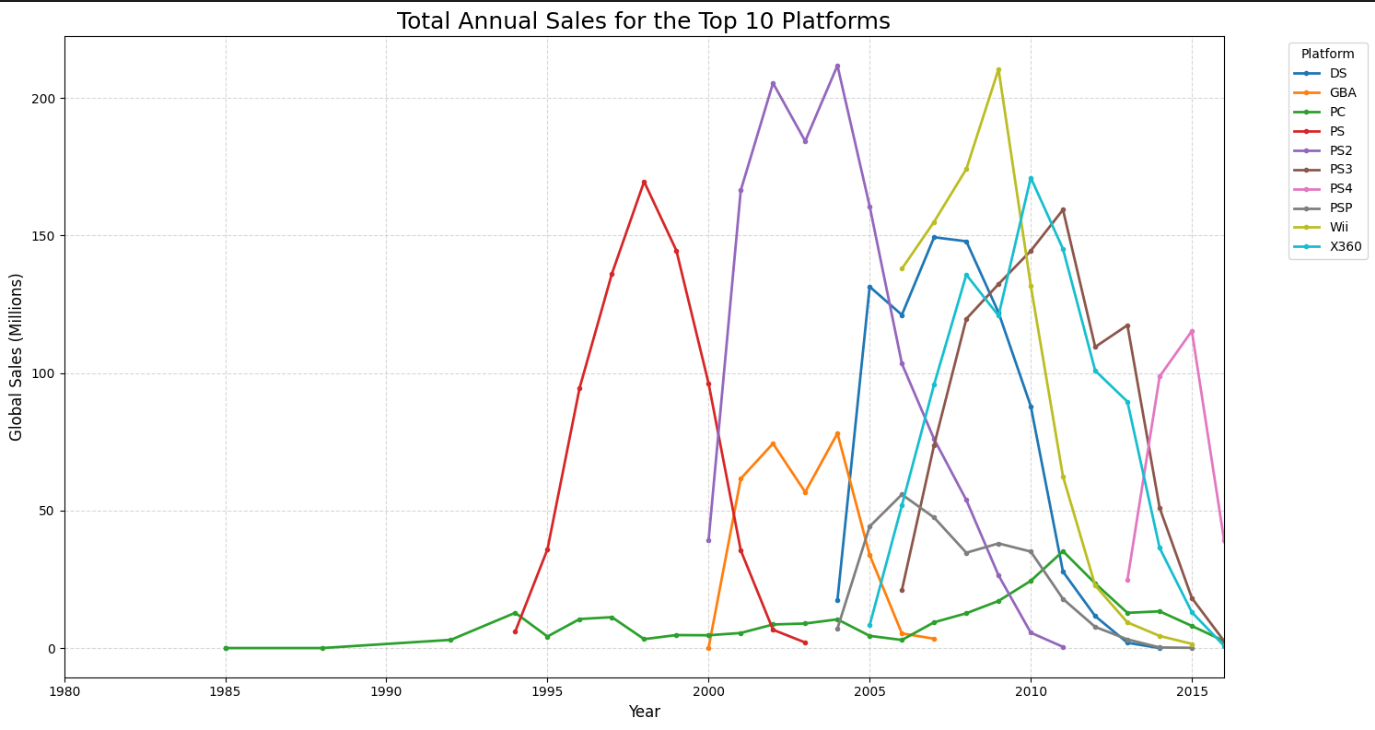
\includegraphics[width=\textwidth]{vgsalesplatovertime.png}
    \end{subfigure}
    \hfill
    \begin{subfigure}[b]{0.2\textwidth}
        \centering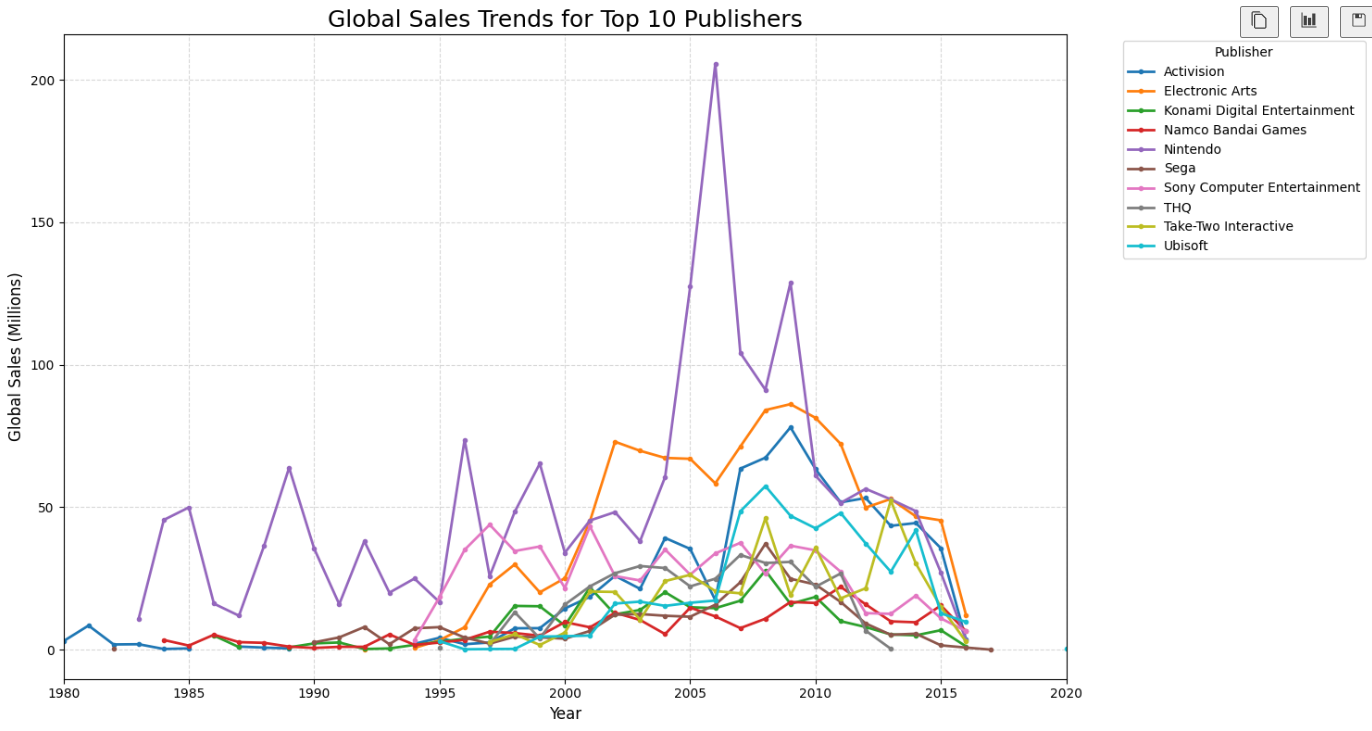
\includegraphics[width=\textwidth]{vgsalespubtime.png}
    \end{subfigure}
\end{figure}
\subsection{Discovery Questions}
\begin{enumerate}
    \item Do publishers do better in their home markets or in
other countries and does the platform or year affect this
outcome? 
    \item Which platforms sold the most video games each year
and were these dominated by specific games or a more
broad spread. 
    \item How have total sales changed over the years in the
different major markets.
\end{enumerate}
\section{Methods}
Three methods were implemented in order to analyze this dataset, these are the K-means and FPGrowth for analysis and Isolation Forest for anomaly detection.
\subsection{Data Preprocessing}
Before any implementations could be made the data needs to cleaned and remove any row that contains an empty column. Other more specific preprocessing is done depending on the implementation.
\subsection{K-means}
There are three different implementations of the K-Means algorithm one for each discovery question. Every K-means implementation used the Elbow method to calculate how many clusters were nessecary.
\subsubsection{First Implementation}
The preprocessing done for this implementation was creating three different percentages  one for each major market in the dataset, this was done for every game in the data set. These percentages where the sales for that market divided by the total sales for that game. This was then run through the K-means algorithm with the 3 percentages and the year of release as each games features.
\subsubsection{Second Implementation}
the preprocessing done for this implementation takes the top seller of a platform in a specific year and divides it by the total sales for that platform that year. These were then run through the K-means.
\subsubsection{Third Implementation}
The preprocessing for this implementation was grouping every game released in a specific year and creating three percentages that divides the total sales in each market that year by the total sales that year. These percentages alongside global sales were then fed into the K-means algorithm.
\subsection{FPGrowth}
The first step in the implementation of the FPGrowth was the creation of three indicators to track whether a game was successful in a market. This was done for all three major markets in the dataset by defining every game that sold more in that market than the median sales in said market. The other indicators would be publisher, platform and the decades the game was released in which was calculated in preprocessing. The three indicators we would track are the market success indicators.
\subsection{Isolation Forest}
The features for the implementation of our Isolation Forest would be the sales in the 3 major markets, Japan, North America, and Europe, Other sales, and Global sales. This allows us to track whether there is any games that do disproportionally well in any of these areas. This allows us to see if any games do well in the any market outside of the main three in this dataset as well which lets us mitigate the problem of some markets not being specified in the dataset.
\section{Results}
\subsection{K-means Analysis}
In this deliverable, we used K-means to analyze the dataset to attempt to answer our 3 discovery questions.
\subsubsection{Question 1: Market Success in Home Market Against Foreign Market}
In addition to the sales, we analyze the characteristics of the clusters including average sales percentage in each market and year, as well as the top 3 consoles in each cluster.
\begin{figure}[H]
    \centering
    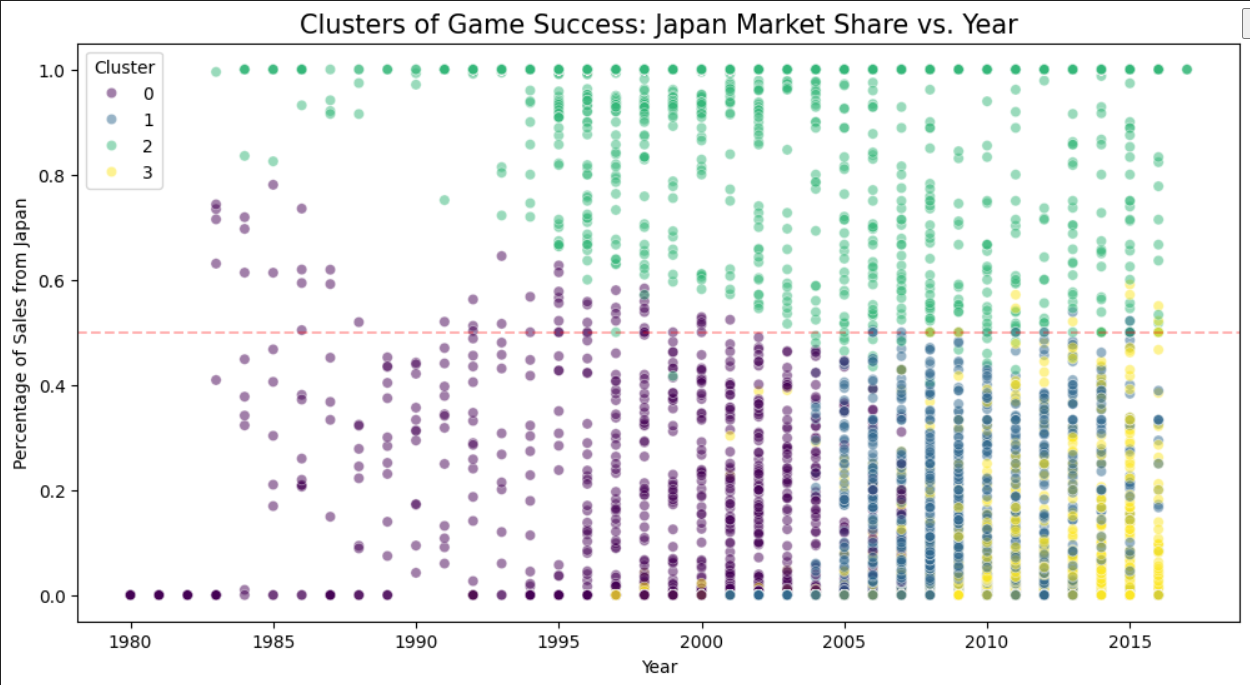
\includegraphics[width=1\linewidth]{kmeasnques1.1.png}
    \label{fig:placeholder}
\end{figure}
\begin{figure}[H]
    \centering
    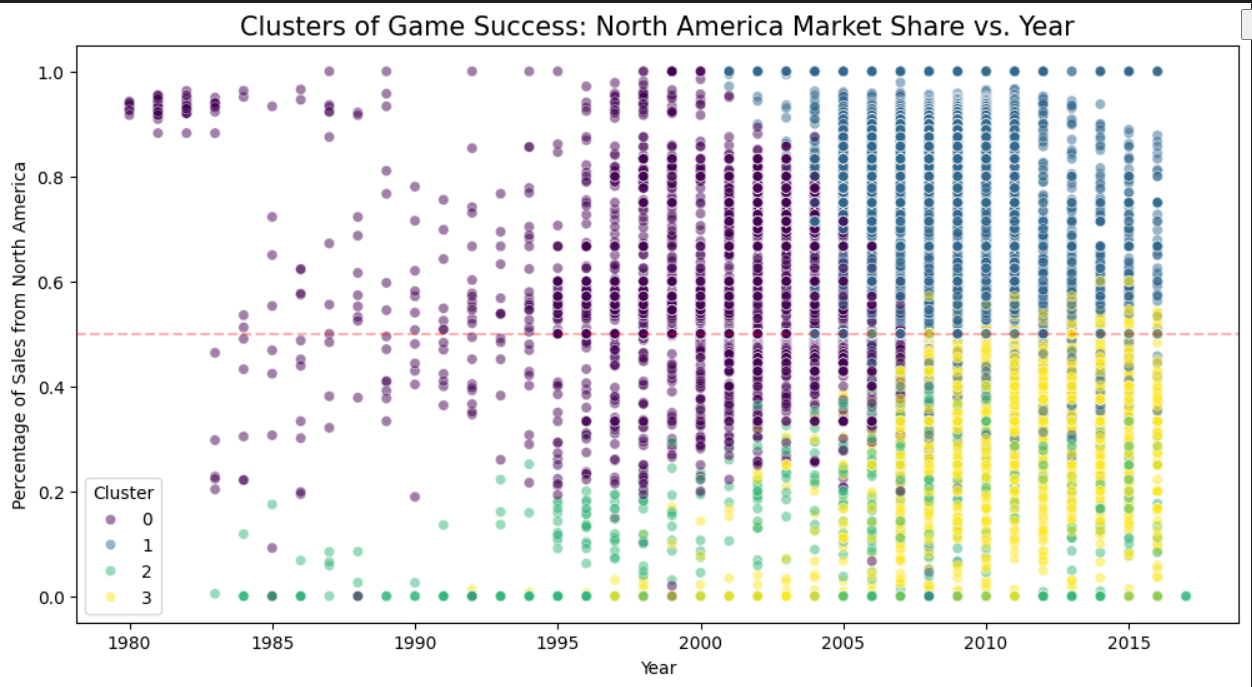
\includegraphics[width=1\linewidth]{kmeansques1.2.png}
    \label{fig:placeholder}
\end{figure}
\begin{figure}[H]
    \centering
    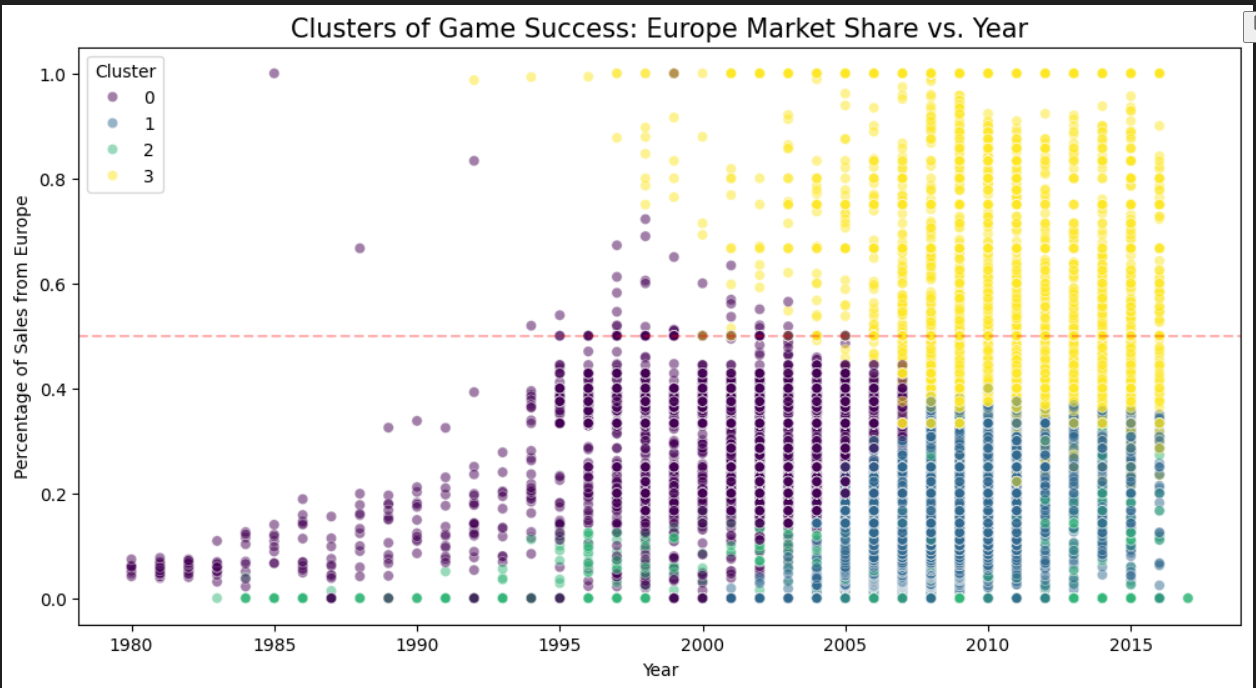
\includegraphics[width=1\linewidth]{kmeansques1.3.png}
    \label{fig:placeholder}
\end{figure}

Cluster 2 shows that there are  a lot of Japanese games that do not make it outside of Japan. Other clusters are more mixed but 2 is overwhelmingly dominated by Japan. Cluster 2's dominant platform were the PSP, DS, and PS2 which are all Japanese consoles showing foreign consoles have a hard time competing with native Japanese ones. Cluster 0 and 1 are both dominated by North American sales,however there is more diversity than in Cluster 2, but have average years of 2000 and 2008 respectively. Cluster 0, the one centered around 2000, has its dominant platforms being the PS, PS2, and GameBoy Advance which shows thatduring this time many North American platforms were struggling to compete against Japanese ones at this time. Cluster 1, the one centered around 2008, has its dominant platforms being the DS, Wii, and Xbox 360 which shows that while Japanese companies still held dominance in the platform market American companies like Microsoft had begun to make moves on the market. Cluster 3 is a European centered cluster while also having the highest average year which shows Europeans have moved into the market more recently compared to the other markets. Cluster 3's dominant platforms were PC PS3 and Xbox 360. This along with the later average year shows that Europeans started buying games more recently than the other markets and had more diversity in platforms with PC allowing dozens of different producers, as well as having both Japanese and American platforms perform well in Europe as well. This shows that in Japan it is difficult for foreign Platforms and therefore publishers to succeed against domestic competition, though this might be due to Sony's and Nintendo's relative dominance in the game industry. North America is still dominated by Japanese platforms, but has some domestic competition allowing for a more diverse ecosystem. Europe is the outlier with PC being the highest platform. This is most likely due to the later average year allowing for Steam to heavily skew the results which shows how dominant the site has become for gaming in recent years. Cluster 2 is the most interesting cluster as it is the only one that has no second place with sales as all other clusters have at least 20 percent of sales outside of the dominant market. This shows Japan has the largest Domestic only game industry with many games likely not releasing outside of Japan while other markets typically have games realeased worldwide alongside their market.
\subsubsection{Question 2: Finding Healthy Platform Ecosystems and Platforms Dominated by Single Games}
\begin{figure}[H]
    \centering
    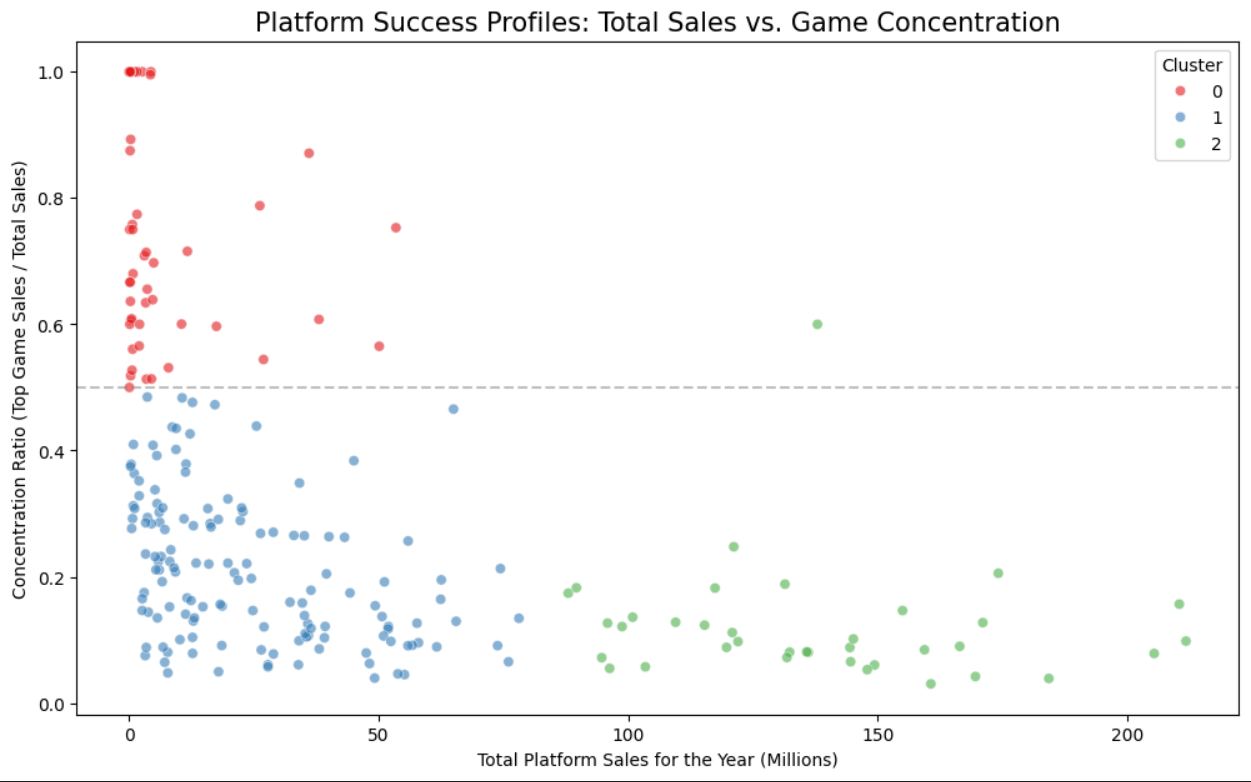
\includegraphics[width=0.8\linewidth]{kmeansques2.png}
    \label{fig:placeholder}
\end{figure}
This analysis has lead to several interesting observations with the 3 clusters. Cluster 0 are platforms that sold poorly that year and only really had one game that pushed its sales up, cluster 1 is platforms that sold poorly that year and had a multitude of games making up its low sales. Cluster 2 is made up of well performing consoles that sold well with lots of games making up the sales. There is one outlier in this cluster though that sold almost 150 million copies with one game making over 60 percent of those sales. There are two outliers in the data those being the ps4 in 2017 and DS in 2020 which both only had one game release in those years in the dataset which shows them as having incredibly unhealthy ecosystems, but for the DS this was well after its life cycle ended and for the PS4 it is likely just a lack of data that skews the results.
\subsubsection{Question 3: Change in Market share Over Time}
\begin{figure}[H]
    \centering
    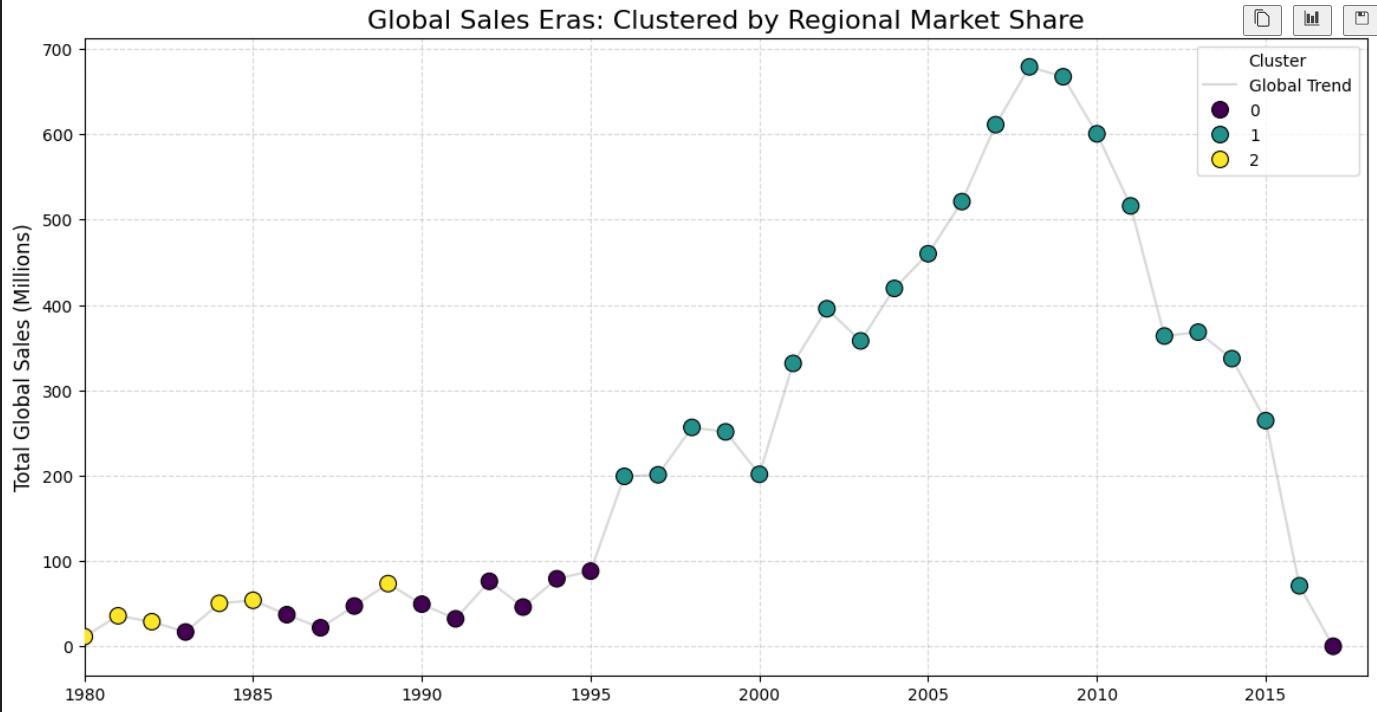
\includegraphics[width=0.8\linewidth]{kmeansques3.png}
    \label{fig:placeholder}
\end{figure}
This analysis was the least insightful of the 3 K-means analysis. There were 3 clusters. Cluster 0 consisted of mainly Japanese sales and shows an era of Japan holding most of the video game market at the start. Cluster 1 is the modern global era of video game sales with high sales all over the world but mainly in North America.  Cluster 2 is dominated by North America with 78 percent of sales being from North America. Cluster 2 has an outlier in 2017 due to the low amount of data in that year. This data shows a shift during the 90's away from Japan as a dominant force in gaming towards North America and finally towards a global market. There is another era starting around 2010 where total sales begin to slump as games begin to take longer to create and less come out.


\subsection{FPgrowth}
\begin{figure}[H]
    \centering
    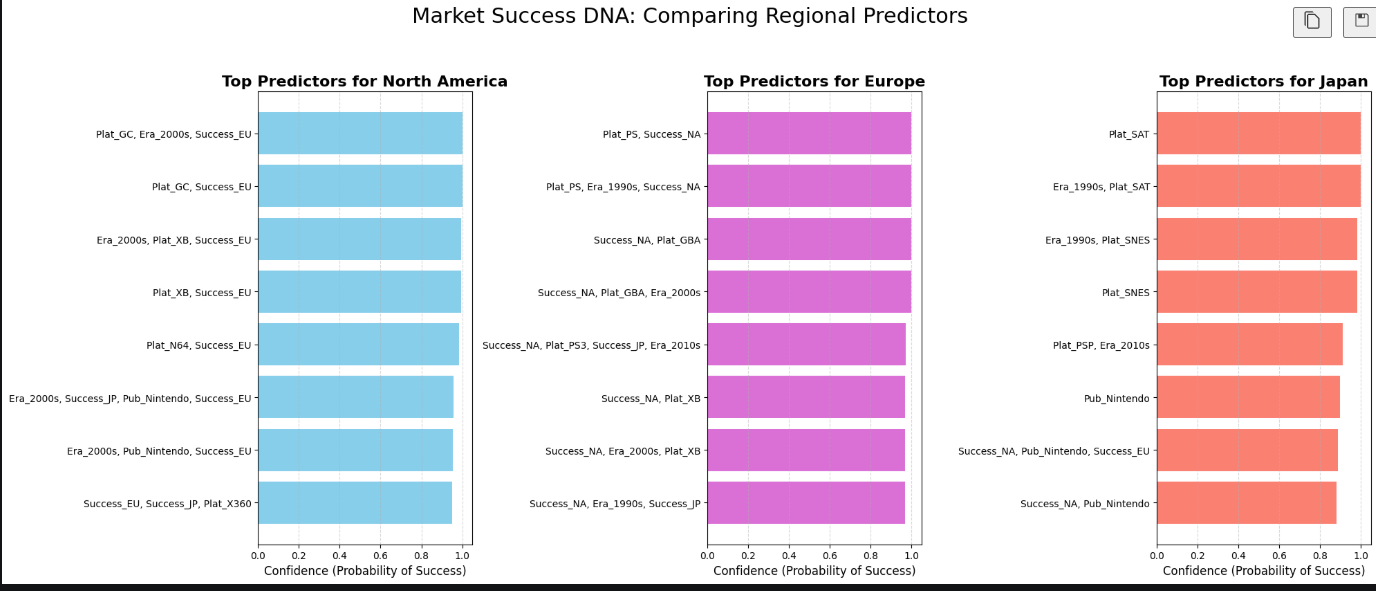
\includegraphics[width=1\linewidth]{DataMiningFPGrowth.png}
    \label{fig:placeholder}
\end{figure}

\subsubsection{Question 1: Market Success in Home Market Against
Foreign Market}
The success in various markets is shown to have very little to do with the publisher of the game. The platform, decade and success in other markets have much more impact on whether or not a game succeeds in a market. The one exception to this is Nintendo as both in North America and Japan where having Nintendo as the publisher allows for around 90 percent of games sell over the median of sales in that region. While in North America this is tied to the 2000s and success in the EU and Japan, Nintendo publishing with no other indicators in Japan allows for around 90 percent of games to perform better than the median while having the game also succeed in North America actually reduces its success rate in Japan. Since Nintendo is based in Japan it actually does prove that some publishers do perform better in their home market than abroad, but since no other publisher appears on the top indicators it shows that Nintendo is an outlier and not the rule especially since it appears so low on the top indicators comparatively to platforms, decades, and success in other markets. Since Nintendo also appears in North America as a success indicator this is further reinforced as it is not just successful in Japan, though success in North America is based on other factors as well further proving that Nintendo is more of an outlier than proof that publishers perform better in their home market.

\subsubsection{Finding Healthy Platform Ecosystems and Successful Platforms}
Indicators for a healthy platform ecosystem in this implementation would be high rates of success for games on a specific platform. There are various platforms shown in the graphs that match this criteria. these include the Game Cube, Xbox, Xbox 360, N64, Playstation, GameBoy Advance, SNES, and surprisingly the Sega Saturn. All of these bar one makes sense as they are some of the most popular consoles of all time meaning they had lots of games and sales. The Xbox seems to be the healthiest across all markets as it is a top indicator for both the North American and European markets. The other platforms only appear in the top 8 indicators in one market. One interesting data point is the Sega Saturn as it failed abroad but was very successful in Japan as releasing on the Saturn as an indicator has 100 percent success rate in Japan with games. It is the only platform that does this without another indicator like success in another market. This outlier could be due to the Sega Saturn's incredible marketing inside Japan compared to outside which helped drive more sales and therefore a healthier platform ecosystem inside Japan compared to its ecosystem in other markets.

\subsubsection{Change in Market share Over Time}
According to indicators of success in the FPGrowth algorithm the 2000s and 1990s have the most successful games as the 2000s appear 5 times in the top 8 of the three markets, and the 1990s appear 4 times. Both these eras are indicators for 100 percent success with both appearing once. The 2010s appear twice showing success is still there but not as much as earlier. This data corroborates the data we found in the k-means as sales began to climb around the 90s and peaked around 2010 before falling by about half and since more success was found in the 1990s and 2000s, 4 and 5 respectively, than the 2010s, only 2 appearances, the data found in the FPGrowth tracks the trend we found previously.
\subsection{Anomaly Detection}

\begin{figure}[H]
    \centering
    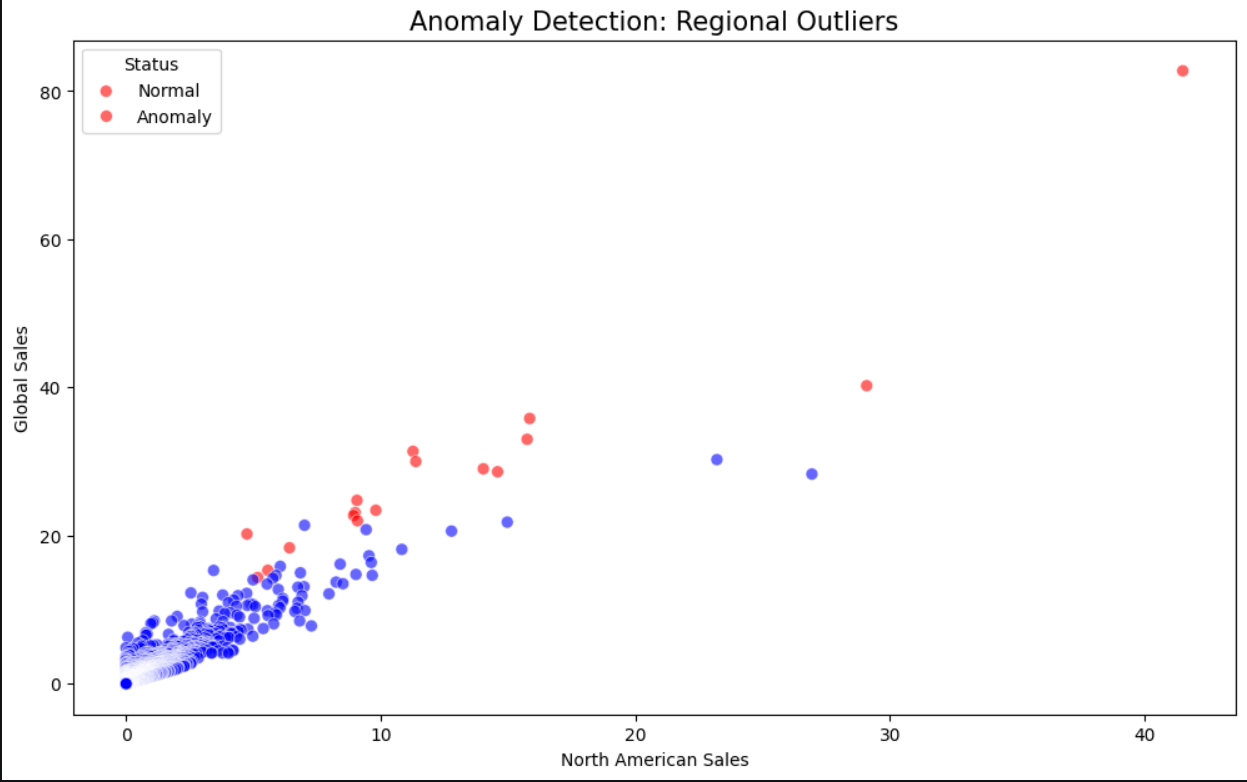
\includegraphics[width=1\linewidth]{DataMiningNAAnomaly.png}
    \label{fig:placeholder}
\end{figure}
\begin{figure}[H]
    \centering
    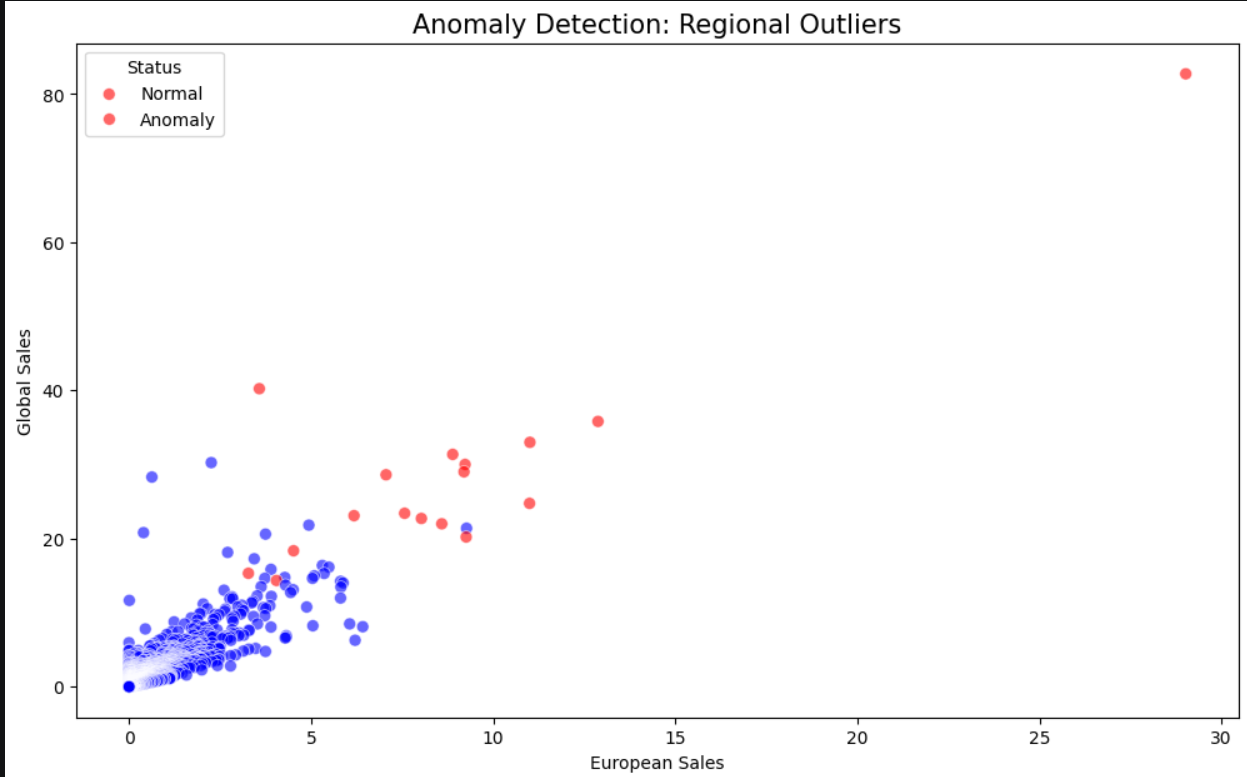
\includegraphics[width=1\linewidth]{DataMiningEUAnomaly.png}
    \label{fig:placeholder}
\end{figure}
\begin{figure}[H]
    \centering
    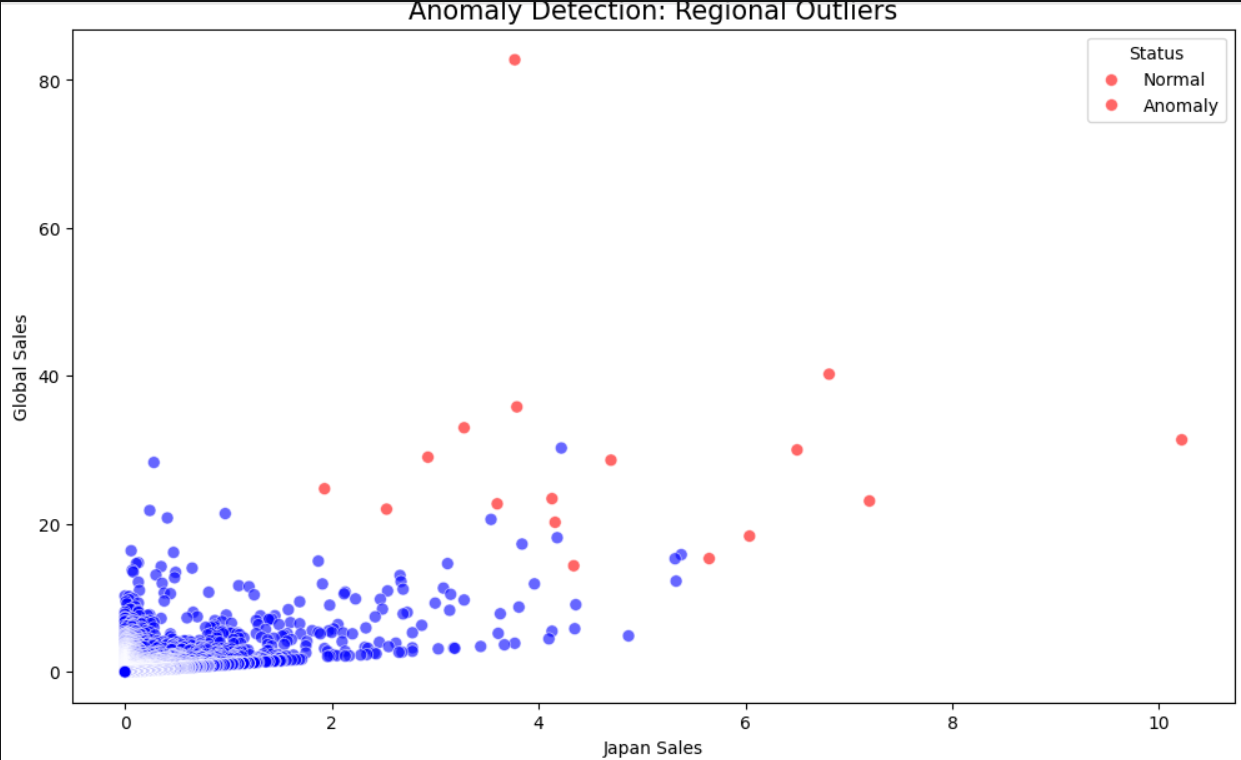
\includegraphics[width=1\linewidth]{DataMiningJPAnomaly.png}
    \label{fig:placeholder}
\end{figure}

The top 10 anomalous data points are all in the top 20 best selling games and all are published by Nintendo. Six of them are Wii games and three are DS games with one being a GameBoy game. All are incredibly well known games like Mario, Wii Sports, or Pokemon with the exception of one that being "Brain Age: Train Your Brain in Minutes a Day" which is the 20th best selling game of all time with most of it coming from Europe which would explain it being flagged as Anomalous. This shows that Nintendo is one of the few publishers that can perform well regardless of market as the anomalous data points are  mostly Nintendo showing they can over perform in markets they typically shouldn't do well in. This shows that while the findings in the FPGrowth show Nintendo performs well in its home region this is less of a symptom of publishers as a whole, but even more evidence that Nintendo is most likely an outlier among publishers.
\section{Critical Assessment}
\subsection{Validity and Limitations}
The data set we used for this analysis is incredibly robust however slightly out of date with only a few games after 2016 and only one in 2020. Many games also are missing the release year data point. even without these games there are still over 11000 games to analyze which gives a robust data pool to allow for trends to be seen. However any trends after 2016 are impossible to track as there is not enough data to work with.
\subsection{Ethics}
The data set used contains data that are publicly available from companies meaning that there are no ethical concerns about taking data from an illegal source.
\section{Conclusion}
\subsection{Question 1:}
The analysis that has been done proves that the publisher of a game has much less effect on the success of a game than I previously thought. There are a multitude of other factors that effect sales much more like platform and release year. The only outlier in this is Nintendo is not only successful in Japan but also North America. While it is more easily able to succeed in Japan than North America this does not prove anything about publishers succeeding in their home market more often as our anomaly detection found Nintendo games to be the most anomalous showing that Nintendo is an outlier likely due to its success with consoles and in house games for said consoles.
\subsection{Question 2:}
The analysis done shows that the top performers every year typically are due to a large volume of games being sold. Even with games like Wii sports being massive outliers in success, incredibly popular consoles tend to have enough other games sell well to create a gaming ecosystem with lots of variety. The top selling consoles each year are typically Nintendo or Sony consoles with the occasional Xbox pushing through to compete.  
\subsection{Question 3:}
The 4 eras we discovered in this analysis are the early era in the 80s where American companies began to make games in the early ages of the video game industry. The second era is the main era of Japanese dominance from the late 80s to mid 90s where most games where sold in Japan before shifting to the third era in the late 90s where the international market opens up and the overall market gets more diverse with Japan falling behind North America and Europe. Finally the final era starts around 2010 where less games start being made and therefore sales begin to slow down but still remain higher than in the 90s.
\subsection{Future Work}
Implementing similar data mining techniques on a more recent database to provide for a more up to date trends of newer platforms and games to check to see if any new trends appear. Expand current analysis on the other sales data point to determine if any trends appear there and what trends continue in this market. 
\end{document}

